\documentclass[titlepage]{article}

\usepackage{preamble}

\title{
    \textbf{ANALYSIS OF \\
    NEURAL NETWORKS \\
    APPLIED TO CONNECT FOUR} \\[0.5cm]
    \rule{10cm}{0.3mm} \\[0.5cm] 
    \small \scshape{A closer look into the intricacies of artificial neural networks} \\[0.4cm]
    \rule{10cm}{0.3mm}
    \vskip -0.3cm
}

\author{
    \small \scshape{Adam Amanbaev, Jonathan Hallström, Alvar Edvardsson} \\ 
    \small \scshape{Hugo Åkerfeldt, Romeo Patzer} \\[0.5cm]
    \small \scshape{Supervisor: Ulf Backlund} \\
    \scriptsize \scshape{Danderyds Gymnasium}
}

\vskip 0.5cm

\begin{document}

\maketitle

\newpage

\begin{abstract}
    In October 2022 DeepMind announced an artificial intelligence in a preprint \cite{alphatensor} that was called AlphaTensor. It utilized \emph{artificial neural networks} and \emph{reinforcement learning} in order to solve the unsolved problem of finding more efficient algorithms for matrix multiplication. AlphaTensor was successful and illustrated the impact of \emph{artificial neural networks} combined with \emph{reinforcement learning}. This paper takes a closer look into the effectiveness of \emph{artificial neural networks} and \emph{reinforcement learning} strategies such as the ones used in AlphaTensor. More precisely, the effects the parameters \emph{kernel size}, \emph{learning rate} and \emph{noise} have on the networks' performance in the board game \emph{Connect Four} are analyzed.

\vskip 1cm

\keywords{Reinforcement Learning, Artificial Neural Network, Deep Learning} 

\end{abstract} 

\newpage

\section*{Preface}

\vskip 0.8cm

\epigraph{
\hspace{2.1cm} The only true wisdom is in knowing you know nothing. 
}
\vskip -0.2cm
\centerline{\scriptsize --Socrates}

\vskip 1.2cm

\subsection*{Background}

\vskip 0.5cm

The concept of artificial intelligence was only popularized during the first half of the 20th century through science fiction. Computers before 1950 lacked key prerequisites for intelligence: they could not store commands, only execute them immediately. In 1956 Allen Newell, Cliff Shaw and Herbert Simon created what is often considered the first artificial intelligence program and it catalyzed the next 20 years of research in this field. 

\vskip 0.3cm

\noindent
Gordon Moore predicted in 1965 that the memory and speed of computers would double every year and the prediction, known as Moore's law, has been true ever since. The growth led to new possibilities for the field of artificial intelligence and many landmark goals were achieved during the 1990's and 2000's. In 1997 reigning world chess champion and grandmaster Gary Kasparov was defeated by IBM's computer program Deep Blue \cite{deep_blue}. 19 years later Deepmind's artificial intelligence AlphaGo \cite{alphago} beat the South Korean grandmaster Lee Sedol regarded as one of the best Go players of all time. Go is due to its large search space considerably more complex than chess and AlphaGo taught itself how to play without any prior knowledge in comparison to Deep Blue which was heavily influenced by pre-coded strategies. Shortly after the success of AlphaGo Deepmind began working on protein structure prediction. The artificial intelligence AlphaFold \cite{alphafold} is now by a huge margin the most accurate in predicting protein structures and it is accelerating research in nearly every field of biology. As the field of artificial intelligence visibly is becoming a substantial part of today's science we find it important to analyze different aspects of it. 

\newpage

\pagenumbering{roman}

\section*{\huge Summary of Notation}
\addcontentsline{toc}{section}{Summary of Notation}

\vskip 0.5cm

\epigraph{
I am a forest, and a night of dark trees: but he who is not afraid of my darkness, will find banks full of roses under my cypresses.
\attr{Friedrich Nietzsche, Thus Spoke Zarathustra}
}

\vskip -1cm

\nomenclature{$\argmin_x f(x)$}{\{$x \mid f(x) = \min_{x'} f(x')$\}}
\nomenclature{$\argmax_x f(x)$}{\{$x \mid f(x) = \max_{x'} f(x')$\}}
\nomenclature{$\leftarrow$}{assignment}

\printnomenclature[3cm]

\newpage

\tableofcontents

\newpage 

\clearpage
\pagenumbering{arabic}

\section{Introduction}

\vskip 0.7cm

\epigraph{
A thinker sees his own actions as experiments and questions--as attempts to find out something. Success and failure are for him answers above all.
\attr{Friedrich Nietzsche}
}

\subsection{Background}

\vskip 0.1cm

Artificial neural networks \cite{ann} are computing systems consisting of connected nodes called artificial neurons and are inspired by biological neural networks that constitute human brains. Artificial networks have recently been used in different forms to solve various complex and abstract problems. A recent example is Deepmind's AlphaTensor \cite{alphatensor} which in October 2022 found a more efficient algorithm for matrix multiplication. 

\vskip 0.3cm

\noindent
The greatest factors of an artificial neural network's success are its architecture and how it is applied to the problem presented. AlphaZero \cite{alphazero} and AlphaGo \cite{alphago} are computer programs whose artificial neural networks only differ in the method of application. Even though AlphaZero uses the same type of network it beats AlphaGo 100 to 0 in the board game Go which demonstrates how delicate artificial networks can be. In this project, we take a closer look at the intricacies of artificial neural networks with the help of the board game Connect Four. We have chosen to study the following aspects: Kernel Size, Learning Rate and Training Noise. The aspects are described further in later sections. 

\subsection{Problem Statement}

\vskip 0.2cm

The following are the questions researched in this paper. The details of the questions are going to be explained in later sections.

\vskip 0.6cm

\begin{outline}
    \1 How does the kernel size in a convolutional network affect the game performance? 
    \1 How does the learning rate in Q-learning affect the game performance? 
    \1 How does training noise affect the self-play training in Q-learning of a network?
\end{outline}

\newpage

\subsection{Delimitations}

\vskip 0.2cm

\subsubsection{Choice of Game}

\vskip 0.2cm

This project is limited to a less complex game due to the limitations of computing power and time. Board games such as Chess or Shogi have large search spaces due to the number of different moves possible from each board state and are therefore not suitable for this project. A board game such as Tic-tac-toe is on the other hand not complex enough to analyze features such as the kernel size of a convolutional neural network. Therefore we chose the board game Connect Four which does not have a too large search space and is complex enough where convolutional kernels can have different effects. 

\subsubsection{Connect Four Implementation}

\vskip 0.2cm

No time will be put into making our Connect Four board user-friendly since it is not the purpose of this project. Time will, on the other hand, be spent making the board and its operations efficient to make training and playing consume less time. 

\subsubsection{Artificial Intelligence}

\vskip 0.2cm

The goal of this project is neither to create a perfect artificial intelligence nor a perfect player. It is rather to analyze what parameters play a role in making an artificial neural network better and what makes it worse. Deficiencies are even welcome as they provide stronger insight into what to avoid when creating and training a neural network. 

\subsubsection{Paper}

\vskip 0.2cm

The purpose of this paper is to inform readers with no prior knowledge about machine learning. It is, therefore, necessary that we concisely present all of the topics from the beginning. Giving a deeper understanding of the theory is a bigger priority for us than presenting formal mathematical descriptions of everything which could end up making the readers more confused. 

\subsection{Outline}

\vskip 0.2cm

Shortly put, the following sections are meant to give the readers enough knowledge to fully grasp the analysis of our project. The last few sections describe our experiment and the process behind it. Furthermore, the results and an analysis of them are presented.

\newpage

\section{Connect Four}

\vskip 0.5cm

\emph{Connect Four} is a two-player connection game, in which two players take turns dropping tokens of their chosen color into a vertically suspended grid with seven columns and six rows. A dropped token takes the lowest available space within the column it was dropped in and the objective of the game is to be the first to form a line of four tokens of the chosen color. Either horizontally, vertically or diagonally. Each player starts the game with 21 tokens of their chosen color. Let the colors, without loss of generality, be black and white and let the player with the black tokens be the first player. If all of the 42 spaces in the grid are filled and none of the players has won the game is drawn. Following are five example games. The first four games are won by the player with white tokens by having created a line of four white tokens vertically, horizontally and diagonally respectively. The last game where both players have used their 21 tokens and not won illustrates a tie.

\vskip 0.75cm

\begin{figure}[h]
    \centering
    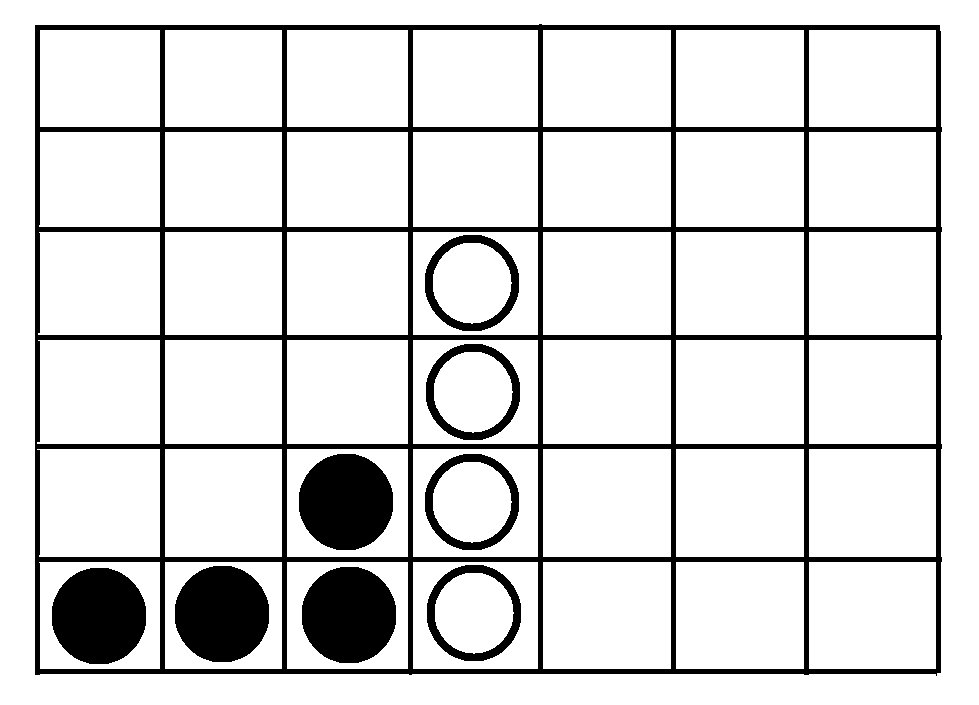
\includegraphics[scale=0.3]{connect4}
    \caption{\scriptsize The player with white tokens wins with four white tokens connected in a line vertically}
\end{figure}

\vskip 0.3cm

\begin{figure}[h]
    \centering
    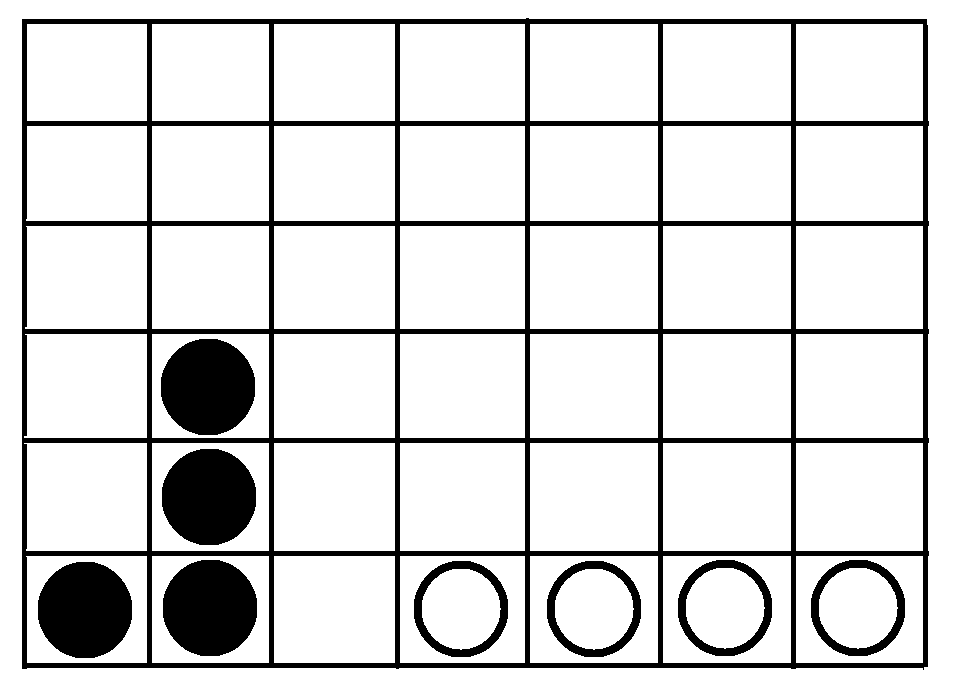
\includegraphics[scale=0.3]{connect4.2}
    \caption{\scriptsize The player with the white tokens wins with four white tokens connected in a line horizontally}
\end{figure}

\newpage

\begin{figure}[h]
    \centering
    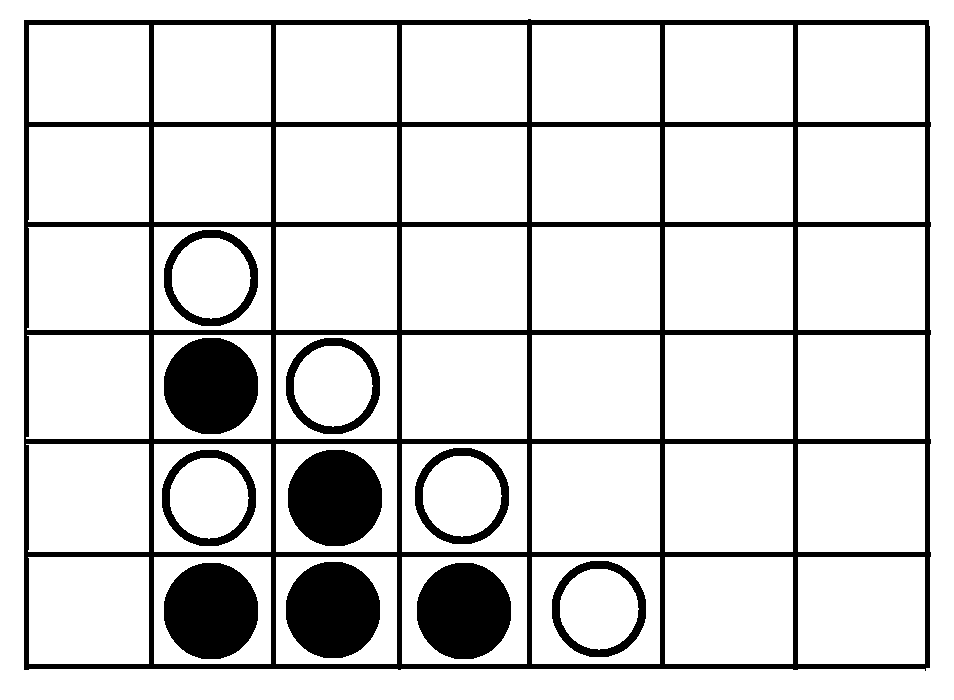
\includegraphics[scale=0.3]{connect4.3}
    \caption{\scriptsize The player with the white tokens wins with four white tokens connected in a line diagonally}
\end{figure}

\vskip 0.3cm

\begin{figure}[h]
    \centering
    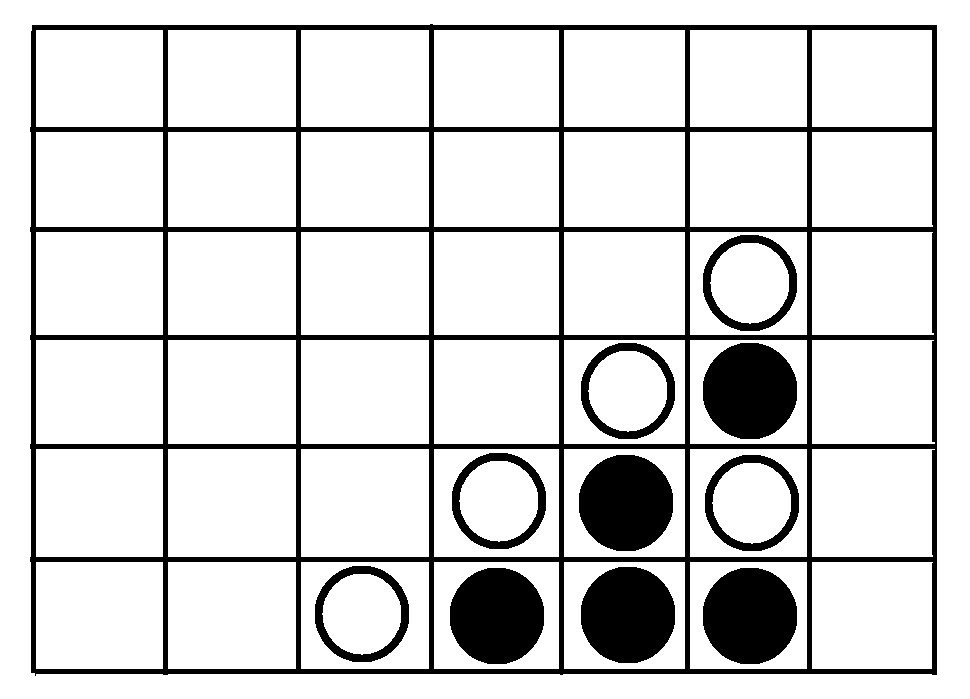
\includegraphics[scale=0.3]{connect4.4}
    \caption{\scriptsize The player with the white tokens wins with four white tokens connected in a line diagonally}
\end{figure}

\vskip 0.3cm

\begin{figure}[h]
    \centering
    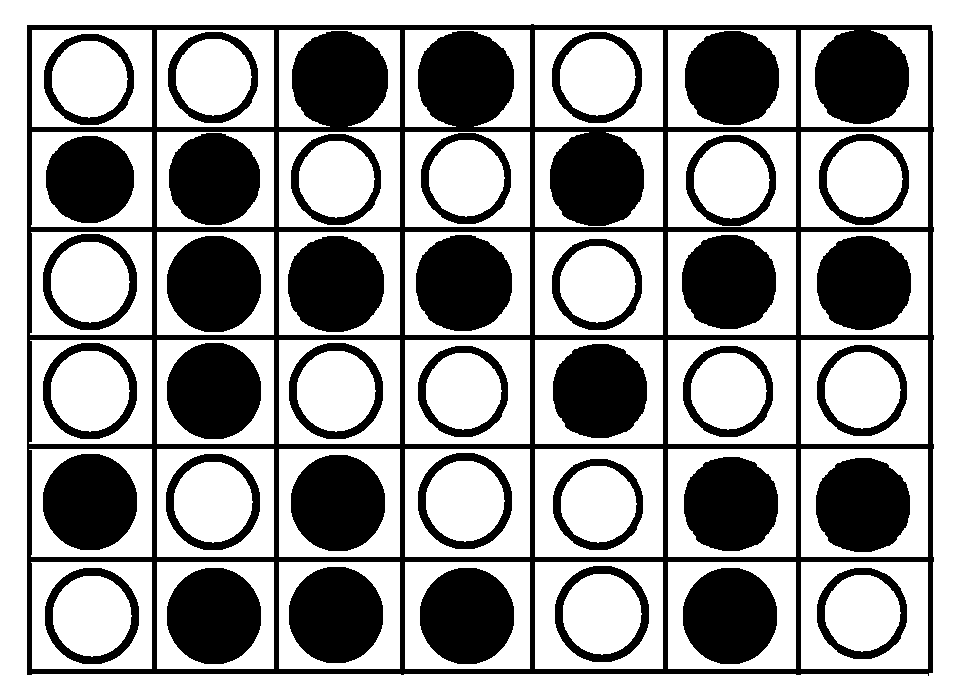
\includegraphics[scale=0.3]{connect4.5}
    \caption{\scriptsize All 42 tokens have been used and no line of four equal-colored tokens was created. It is therefore a tie.}
\end{figure}

\newpage

\section{Reinforcement Learning}

\vskip 0.5cm

\epigraph{
Action comes about if and only if we find a discrepancy between what we are experiencing and what we want to experience.
\attr{Philip J. Runkel}
}

\subsection{Introduction}

\vskip 0.3cm

The nature of learning is often associated with the foundational idea of learning by interacting with the surrounding environment. When a child learns how to ride a bicycle, the child either falls or manages to stay in balance. Every time parents speak to their children they indirectly correct the children's sentences by repeating them correctly. Constantly interacting with the environment produces a wealth of information about the consequences of actions, their cause and effect of them and what actions to take to achieve a certain goal. These kinds of interactions undoubtedly play a major role throughout our lives as we learn about ourselves and the environment surrounding us. Whether it is learning how to ride a bike or how to speak, we are always aware of how the environment responds to our actions. By behaving in a certain manner and choosing actions carefully, we can reach the goals we seek. Reinforcement learning \cite{sutton} offers a computational approach to learning from interaction. By primarily exploring idealized learning situations and evaluating the effectiveness of various learning methods, reinforcement learning focuses a lot more on goal-oriented learning from interaction than any other machine learning approach. 

\subsection{Examples}

\vskip 0.3cm

The following are examples to better grasp the concept of reinforcement learning and how it could be applied to real-life problems.

\vskip 0.3cm

\begin{outline}
    \1 Adam left his house five minutes ago and is on his way to school. He suddenly starts questioning whether he locked the front door or not. Turning home would at this point make him late to class but leaving the house unlocked has its risks. Adam makes his decision based on the time he gets home after school and how often he has forgotten to lock the door. 
    \1 Hugo is playing chess against the current chess world champion Magnus Carlsen. In order not to lose, Hugo makes moves by evaluating the current position intuitively, and anticipating possible counterreplies. Since Hugo is familiar with the current position and has played it at home several times, he is quite confident in his decisions. 
    \1 Romeo could hardly move his body the first few months after being born. One year later, he was running at 1.6 meters per second.
    \1 Jonathan is in a casino and suddenly sees ten slot machines. He does not know the probability of getting a jackpot on any of the machines but knows the cost of each lever pull and the reward given by a jackpot. Through repeated selections of slot machines, Jonathan manages to maximize his winnings by concentrating on the best levers. 
    \1 Alvar is cleaning his very large house. It is so large that he needs to refuel his body with cereal in order to clean everything. Before entering a new room to clean, Alvar decides whether he should start trying to find his way back to the kitchen where the cereal is or pick up the trash in the new room. Alvar makes his decision based on how tired he feels and how quickly and easy he has been able to find his to way to the kitchen in the past.
\end{outline}

\vskip 0.2cm

\noindent
All of the examples share features that are easily overlooked due to their simplicity. They all involve interaction between a decision-making agent and an environment, where the agent is trying to achieve a particular goal without knowing the full extent of the environment, nor the consequences of its actions. The agent's actions can affect the environment (e.g., Hugo making a move against Magnus Carlsen changes the state of the board) thereby affecting the actions available to the agent in the future. None of the actions, in all of the examples, can be predicted fully and the agent must instead observe the environment and how it changes based on actions to learn how to properly behave. 

\subsection{Elements of Reinforcement Learning}

\vskip 0.3cm

As previously illustrated, there are two primary components of reinforcement learning, an agent and an environment. It is, on the other hand, possible to recognize three more elements of a reinforcement learning system. These being a policy, a reward signal, and a value function. 

\vskip 0.3cm

\noindent
A \emph{policy} \cite{sutton} describes an agent's way of deciding actions at given times. It could roughly be defined as a mapping from a state of the environment to actions to be taken at that state. 
\vskip 0.3cm

\noindent
Further, the \emph{reward signal} \cite{sutton} determines the goal of the learning agent. After each decision the agent makes, the environment sends a reward signal, and the goal is to maximize the total reward after all of the actions have been made. The reward signal thus determines what actions are good and bad, respectively. This is comparable to pain and pleasure in human beings. When a child falls off their bike, they receive a negative reward signal in the form of pain. On the other hand, maintaining balance on the bike for a certain amount of time sends a positive reward signal in the form of happiness. Since the child, the learning agent, wants to experience joy instead of pain, the goal becomes riding a bike without falling off it. 

\vskip 0.3cm

\noindent
Lastly, whereas the reward signal immediately tells the agent whether an action was good or bad, the \emph{value function} \cite{sutton} tries to tell whether an action is good or bad in the long run. It could roughly be defined as the expected total reward after a certain action while a reward signal only informs the agent about the immediate reward. 

\subsection{Markov Decision Process}

\vskip 0.2cm

A Markov Decision Process \cite{sutton}, MDP, is a more rigorous and mathematical way of describing a sequential decision-making system. An MDP can formally be defined as MDP$(S, A, R)$ where each parameter is defined as follows:

\vskip 0.3cm

\begin{outline}
    \1 $S$ is the set of all the possible states the environment take on.
    \1 $A$ is the set of all possible actions that can be taken within the environment.
    \1 $R$ is the set of numerical reward signals returned for each action taken by the agent.
\end{outline}

\begin{figure}[h]
    \centering
    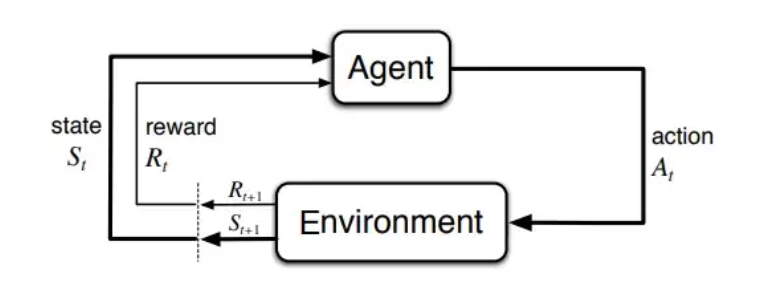
\includegraphics[scale=0.6]{MDP}
    \caption{Illustration of Markov Decision Process}
\end{figure}

\noindent
More specifically, an agent and an environment interact with each other in an MDP at discrete time steps, $t = 0, 1, 2, 3, ...$. The agent receives a representation of the environment's state, $S_{t} \in S$, at each time step and accordingly selects an action, $A_{t} \in A(S)$. The time step following, $t + 1$, as a consequence of its action, the agent receives a reward signal, $R_{t} \in R$, and arrives at a new state, $S_{t+1}$. The MDP thereby gives rise to the following sequence: 

\vskip 0.3cm

\centerline{$S_{0}, A_{0}, R_{1}, A_{1}, R_{2}, S_{2}, A_{2}, R_{3}, ...$}

\vskip 0.3cm

\noindent
In our case, with Connect Four, the board becomes the environment, and the players are agents taking turns interacting with it in the Markov Decision Process.

\subsection{Q-Learning}

\vskip 0.2cm
In 1989 Watkins \cite{sutton} released one of the early breakthroughs in reinforcement learning. It was the algorithm known as Q-learning which is a way for an agent to learn how to optimally navigate in a Markov Decision Process (3.4). The Q-learning algorithm is an action-value function which maps actions to values, where the action values are called Q-values. The Q-learning algorithm evaluates how beneficial a certain action is in a given situation and a higher Q-value corresponds to a better action. The evaluations made by the algorithm improve over time. The algorithm \cite{sutton} is formally defined as follows:

\newpage

\begin{figure}[h]
    \centerline{$Q_{new}(S_{t}, A_{t}) \leftarrow Q(S_{t}, A_{t}) + \alpha[R_{t+1} + \gamma\max_{a}Q(S_{t+1}, a) - Q(S_{t}, A_{t})]$}
    \vskip 0.2cm
    \caption{The Q-learning algorithm}
\end{figure}

\vskip 0.3cm

\noindent
\emph{Gamma}, $\gamma$, is in this expression known as the discount factor and it changes the behaviour in the agent's actions. Values closer to 0 lead to the reward $R_{t}$ propagating worse from the state $S_{t}$ to $S_{0}$ which encourages the agent to take actions that yield immediate rewards. A discount factor closer to the value 1 will on the other hand encourage the agent to take actions that yield later rewards since a larger portion of the reward propagates through the states in this case. 

\vskip 0.3cm

\noindent
\emph{Alpha}, $\alpha$, is in this expression known as the learning rate and regulates the agent's rate of learning, just as the name suggests. Values closer to 0 will decrease the update in the formula. A learning rate closer to 1 will, on the other hand, increase the rate of learning as a large part of the updated value remains.

\vskip 0.3cm

\noindent
The algorithm assigns a new value, $Q_{new}(S_{t}, A_{t})$, to the action-value mapping where $Q(S_{t}, A_{t})$ is the current value for the action $A_{t}$ at the state $S_{t}$. It also makes use of $\max_{a}Q(S_{t+1}, a)$, which is the largest Q-value amongst all actions from the state $S_{t+1}$. 

\subsection{Double Q-Learning}

\vskip 0.2cm

Since the future maximum action value, $\max_{a}Q(S_{t+1}, a)$, in Q-learning is evaluated using the same Q functions as the one used by the agent to choose the action, $a_{t}$, the algorithm risks overestimating certain action values \cite{doubleq}. In our case with Connect Four, it could be evaluating bad moves that randomly led to a victory the same as good moves that lead to a victory. This slows down the learning since the Q-learning algorithm will later need to re-adjust the overestimated evaluations. A variant called double Q-learning \cite{doubleq} was proposed to correct this. In practice, it uses two separate value functions, $Q_{X}$ and $Q_{Y}$, that are updated in a mutually symmetric fashion using each other. Double Q-learning is defined as follows:

\vskip 0.5cm

\begin{figure}[h]
    \centerline{$Q^X(S_{t}, A_{t}) \leftarrow Q^X(S_{t}, A_{t}) + \alpha[R_{t} + \gamma Q^Y(S_{t+1}, \argmax_{a}Q^X(S_{t+1}, a)) - Q^X(S_{t}, A_{t})]$}
    \vskip 0.5cm
    \centerline{$Q^Y(S_{t}, A_{t}) \leftarrow Q^Y(S_{t}, A_{t}) + \alpha[R_{t} + \gamma Q^X(S_{t+1}, \argmax_{a}Q^Y(S_{t+1}, a)) - Q^Y(S_{t}, A_{t})]$}
    \vskip 0.2cm
    \caption{The double Q-learning algorithm}
\end{figure}

\vskip 0.3cm

\noindent
Now that the future maximum action is evaluated using a separate value function the overestimation issue has been solved. The double Q-learning algorithm could be seen as two people checking that each other's homework is done correctly which naturally increases the correctness and in turn the effectiveness.

\newpage

\section{Deep Learning}

\subsection{Introduction}

\vskip 0.2cm

Deep learning is a machine learning method based on artificial neural networks \cite{deeplearning}. Details about the artificial neural networks used in this project are presented in the following sections. 

\subsection{Basic Architecture of Neural Networks}

\vskip 0.2cm

Artificial neural networks \cite{charu} are simulations of the mechanism of learning in biological organisms. The human brain and nervous system contain cells known as neurons. The neurons are connected with the help of synaptic connections. The strength of the synaptic connections changes in response to external stimuli, which is how learning takes place, not only in humans but also in many other living organisms. 

\vskip 0.3cm

\noindent
This learning is simulated in artificial neural networks \cite{charu} which contain artificial neurons. The neurons are connected through weights that imitate the strength of synaptic connections in living organisms.

\vskip 0.3cm

\noindent
We will from here on out refer to artificial neural networks as \emph{neural networks} and not the neural networks in living biological creatures. Furthermore, artificial neurons will be referred to as \emph{nodes}.

\vskip 0.5cm

\begin{figure}[h]
    \centering
    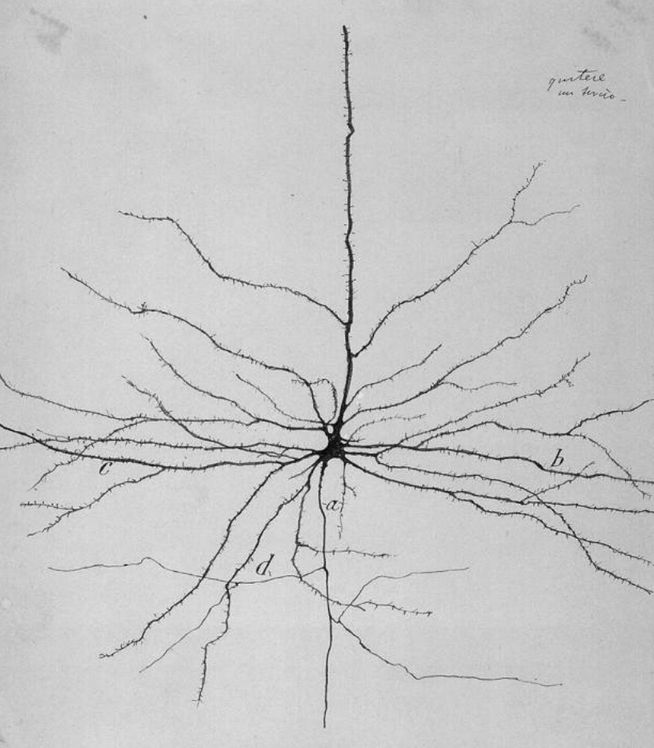
\includegraphics[scale=0.35]{neuron}
    \caption{A typical neuron and its synaptic connections}
\end{figure}

\subsubsection{Perceptron}

\vskip 0.2cm

The simplest neural network is the perceptron \cite{charu} and it consists of a single input layer and an output node. 

\begin{figure}[h]
    \centering
    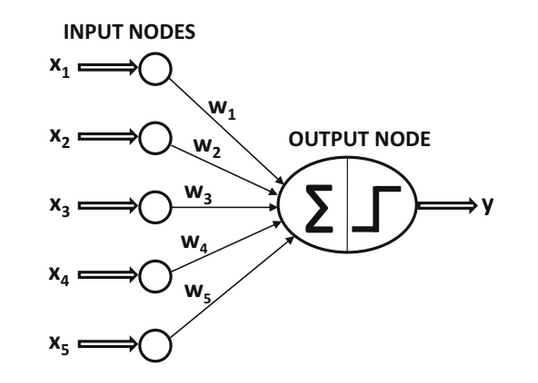
\includegraphics[scale=0.5]{perceptron}
    \caption{The basic architecture of the perceptron}
\end{figure}

\vskip 0.1cm

\noindent
The basic architecture of the perceptron is shown in Figure 10 above. The input layer consists of input nodes that each are connected to the output node through weights, $w_{1}, w_{2}, ..., w_{6}$. The input nodes do not perform any changes to the input values, $x_{1}, x_{2}, ..., x_{6}$ and send the input values to the output node through the corresponding weight connections. The output node then receives the sum of each input value multiplied by the weight it was sent through, a weighted sum. The node also contains an internal value called \emph{bias}, $b$, that is added to the sum. If we let $v$ denote the output node's recieved value, then $v = b + \sum w_{i} x_{i} = w_{1} x_{1} + w_{2} x_{2} + ... + w_{6} x_{6}$. Before the output then sends the value further, it applies an \emph{activation function} which often is non-linear. If we let $f$ denote the activation function, the output of the output node becomes $y = f(v)$. This procedure where a set of input values, $x_{i}$ are transformed into a set of output values, $y_{i}$, by the neural network is called a \emph{forward pass} \cite{charu}.

\subsubsection{Multilayered Neural Network}

\vskip 0.2cm

Multilayer neural networks consist of more than one computational layer \cite{charu} in contrast to the perceptron. The perceptron only consists of an input and output layer, whereas the output layer is the only layer that performs computations. Multilayer neural networks on the other hand contain intermediate layers in addition to the input and output layers. The intermediate layers are between the input and output layers and are often referred to as \emph{hidden layers} since the computations performed by them are not visible. The weight connections, internal biases and the mechanics of the forward pass remain the same as in the perceptron, the only difference being that there are several nodes in each hidden layer which receive a weighted sum of values from the preceding layer.

\newpage

\begin{figure}[h]
    \centering
    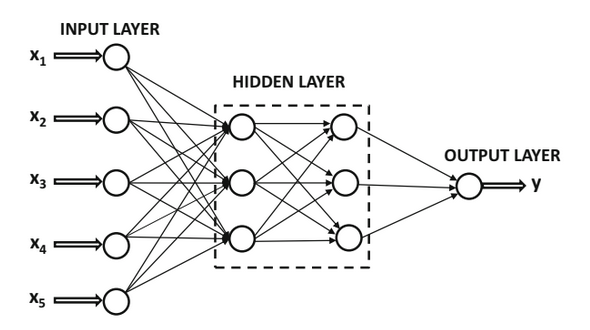
\includegraphics[scale=0.6]{multilayered}
    \vskip 0.2cm
    \caption{The basic architecture of a multilayered neural network with two hidden layers and a single output layer. Note that the input layer is excluded when we count the number of layers since it only transmits the input data into the network. }
\end{figure}

\vskip 0.3cm

\noindent
In the default multilayered neural network \cite{charu} each node in one layer is assumed to be connected to each of those of the next layer, as shown in Figure 11 above. The layers used in the default multilayer neural network are also often referred to as \emph{fully connected layers}. Each layer except the input layer applies an activation function to the value of each node before passing them forward to the next layer. These activation functions can differ between layers but only one is in practice used for each node in a layer.

\vskip 0.2cm

\subsubsection{Example}

\begin{figure}[h]
    \centering
    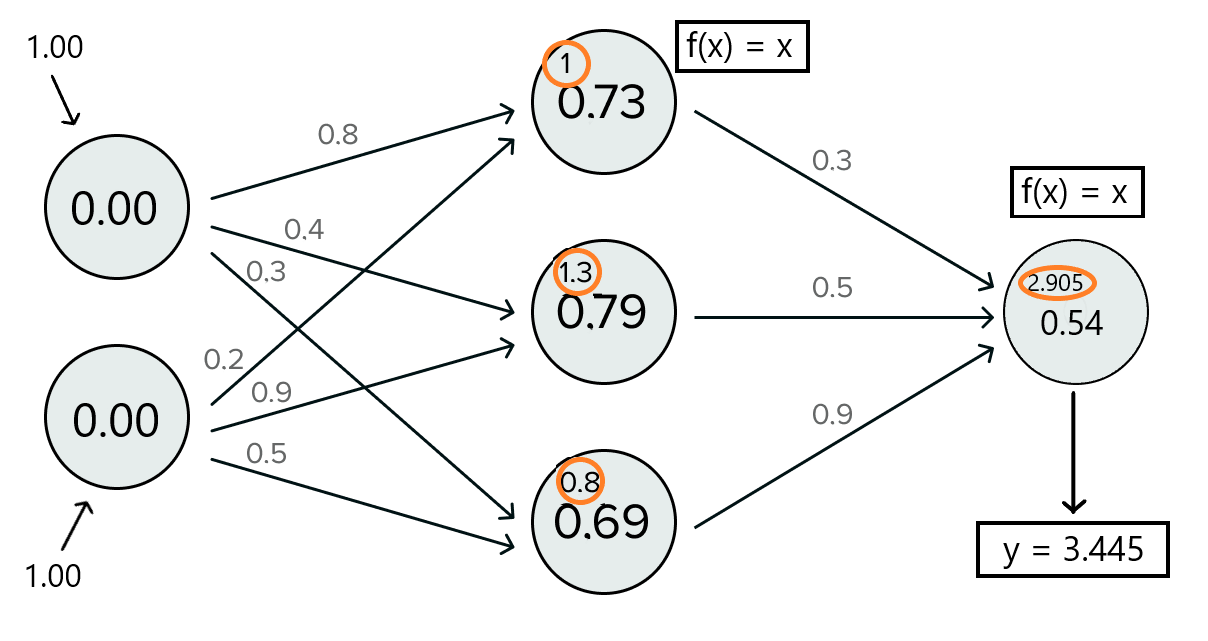
\includegraphics[scale=0.3]{feedforward}
    \caption{A forward pass in a multilayer neural network with 1 hidden layer and 1 output layer. Weighted sums from the preceding layers are in orange. The value in each node represents its internal bias.}
\end{figure}

\noindent
Figure 12 above illustrates a multilayer neural network with 2 input nodes, followed by a hidden layer with 3 nodes which connects to a single output node. Both the hidden and the output layers use a linear activation function, $f(x) = x$, for simplicity. The two input values are each 1 and the internal bias, $B$, of input nodes is always 0. Let each node be indexed as $(i, j)$ where $i$ is the index of the layer from left to right, zero-indexed, and $j$ is the index of the node in its layer from top to bottom, zero-indexed. Furthermore let $W_{(i_{1}, j_{1}) (i_{2}, j_{2})}$ denote the weight connection between node $(i_{1}, j_{1})$ and $(i_{2}, j_{2})$. The value, $V$, of each node and the final output, $y$, are then calculated as follows: 

\vskip 0.8cm

\centerline{$V_{(0, 0)} = 1.0 + 0.0 = 1.0$}

\vskip 0.2cm

\centerline{$V_{(0, 1)} = 1.0 + 0.0 = 1.0$}

\vskip 0.5cm

\centerline{$V_{(1, 0)} = B_{(1, 0)} + W_{(0, 0) (1, 0)} V_{(0, 0)} + W_{(0, 1) (1, 0)} V_{(0, 1)} = 0.73 + 0.8 * 1.0 + 0.2 * 1.0 = 1.73$}

\vskip 0.2cm

\centerline{$V_{(1, 1)} = B_{(1, 1)} + W_{(0, 0) (1, 1)} V_{(0, 0)} + W_{(0, 1) (1, 1)} V_{(0, 1)} = 0.79 + 0.4 * 1.0 + 0.9 * 1.0 = 2.09$}

\vskip 0.2cm

\centerline{$V_{(1, 2)} = B_{(1, 2)} + W_{(0, 0) (1, 2)} V_{(0, 0)} + W_{(0, 1) (1, 2)} V_{(0, 1)} = 0.69 + 0.3 * 1.0 + 0.5 * 1.0 = 1.49$}

\vskip 0.5cm

\centerline{$V_{(2, 0)} = B_{(2, 0)} + W_{(1, 0) (2, 0)} f(V_{(1, 0)}) + W_{(1, 1) (2, 0)} f(V_{(1, 1)}) + W_{(1, 2) (2, 0)} f(V_{(1, 2)}) =$}

\vskip 0.2cm

\centerline{$V_{(2, 0)} = B_{(2, 0)} + W_{(1, 0) (2, 0)} V_{(1, 0)} + W_{(1, 1) (2, 0)} V_{(1, 1)} + W_{(1, 2) (2, 0)} V_{(1, 2)} =$}

\vskip 0.2cm

\centerline{$0.54 + 0.3 * 1.73 + 0.5 * 2.09 + 0.9 * 1.49 = 3.445$}

\vskip 0.5cm

\centerline{$y = f(V_{(2, 0)}) = V_{(2, 0)} = 3.445$}

\vskip 1cm

\subsubsection{Choice of Activation Function}

\vskip 0.2cm

Figure 12 shows a neural network that only uses a linear activation function, $f(x) = x$, but non-linearity must be introduced into the network. Non-linearity means that the output of the neural network cannot be reproduced from a linear combination of the input values. Without a non-linear activation function in the neural network, no matter how many layers it has, it would behave like a simple perceptron, since combining the layers would only produce another linear function. By introducing non-linear activation functions into the neural network, it can approximate models that vary non-linearly in addition to linear models. The activation function used throughout this project is the hyperbolic tangent function, \emph{tanh}, which has the output range $[-1, 1]$ and is defined as follows:

\vskip 0.4cm

\begin{figure}[h]
    \centerline{$\tanh(x) =$ \scalebox{1.5}{$\frac{e^x - e^{-x}}{e^x + e^{-x}}$}}
    \vskip 0.2cm
    \caption{The hyperbolic tangent function}
\end{figure}

\vskip 0.2cm

\noindent
The activation function needs to be defined and differentiable for reasons described in later sections.

\newpage

\subsection{Interpretation}

\vskip 0.2cm

A neural network can be interpreted as a large statistical model with a large number of parameters, and weight connections. If each of the parameters, weight connections, were to be tuned well, then the model would be able to represent highly abstract and complex correlations. A less rigorous way of imagining this would be having a function in a space with as many dimensions as weight connections in the network. The phenomena that that function would be able to approximate would be beyond our understanding. This leads to the most common usage of neural networks. Namely training neural networks by adjusting their weight connections for it to approximate a certain function with the help of data. An example would be approximating the sinus curve with a neural network. By giving an x-coordinate as input to the network and comparing the network's output value with the y-coordinate one only needs to adjust the weight connections of the network in such a manner that the error decreases to make it a better approximation. This is further described in the following sections.

\vskip 0.5cm

\begin{figure}[h]
    \center
    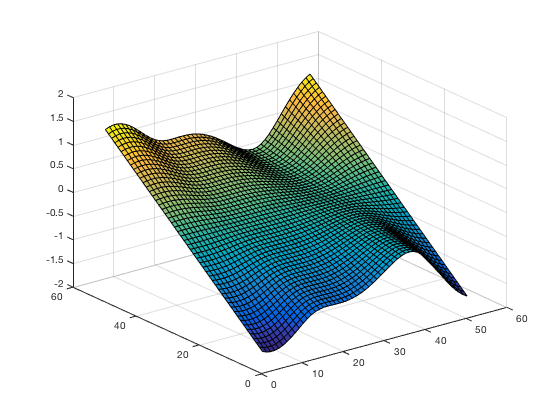
\includegraphics[scale=0.5]{twodim}
    \vskip 0.3cm
    \caption{A 3-dimensional graph that could easily be approximated by a neural network with 2 input nodes}
\end{figure}

\vskip 0.2cm

\noindent
The 3-dimensional graph shown in Figure 14 above is quite complex but can still be approximated by a small neural network with only 2 input nodes. However, a neural network usually has up to hundreds of input nodes and can train to represent even more complex models.

\newpage

\subsection{Training a Neural Network}

\vskip 0.5cm

\epigraph{
Repetition is the mother of learning, the father of action, which makes it the architect of accomplishment. 
\attr{Zig Ziglar}
}

\subsubsection{Loss Function}

\vskip 0.2cm

To be able to train a neural network to a certain level we, first of all, need to know at what level it currently is. An efficient method to measure this is to find an error. Given an output target and the neural network's output, the error can be described as a function of them. To then improve the network we simply need to find a way to decrease that error. This type of function which is to be minimized is also referred to as a \emph{loss function} \cite{charu}. How the loss function is used to train a neural network is described in later sections. The loss function used throughout this project is the \emph{Mean Squared Error} \cite{charu}, MSE, and is defined over a set of network predictions or outputs, $\hat{y_{1}}, \hat{y_{2}}, ..., \hat{y_{n}}$, and output targets, $y_{1}, y_{2}, ..., y_{n}$ as follows:

\vskip 0.5cm

\begin{figure}[h]
    \centerline{\scalebox{1.3}{$MSE = \frac{1}{n}\sum_{i=1}^{n}(y_{i} - \hat{y_{i}})^2$}}
    \vskip 0.2cm
    \caption{The Mean Squared Error loss function}
\end{figure}

\vskip 0.3cm

\noindent
An advantage of The MSE is that it ensures that our trained model will not have outlier predictions with prominent errors, since the MSE puts larger weight on those errors due to the squaring in the function. A disadvantage is, on the other hand, that a single very poor prediction made by the network will overly impact the training since the error is magnified by the squaring part of the MSE function. Since most of the cases aim for more of a well-rounded neural network that performs well on most of the data those outliers should be ignored and not prioritized. This is not a big problem in our project since our networks only output values in the range $[-1, 1]$ which ensures that the squaring in the MSE does not magnify any errors by a lot.

\newpage

\subsubsection{Descending the Loss Function}

\vskip 0.2cm

Assume we are trying to train a perceptron with one input node and one output node with one weight connection, $w$, between them. For the sake of simplicity, let the output node's activation function be linear, $f(x) = x$. Let the input value be a constant $x$, the output target be a constant $y$, and the output node's internal bias be a constant $b$. The error is then defined as follows: 

\vskip 0.5cm

\centerline{$MSE = \frac{1}{1}\sum_{i=1}^{1}(y_{i} - \hat{y_{i}})^2 = (y - f(V_{(1, 0)}))^2 = (y - V_{(1, 0)})^2 = (y - (b + w * x))^2$}

\vskip 0.5cm

\noindent
Notice that $w$ is the only variable in the error and is exactly what needs to be adjusted as mentioned in section 4.3. If we now plot the MSE function as a function of $w$ things become more apparent. The second-degree polynomial created by the MSE in respect to the weight, $w$, is illustrated below, non-scaled:

\vskip 0.5cm

\begin{figure}[h]
    \center
    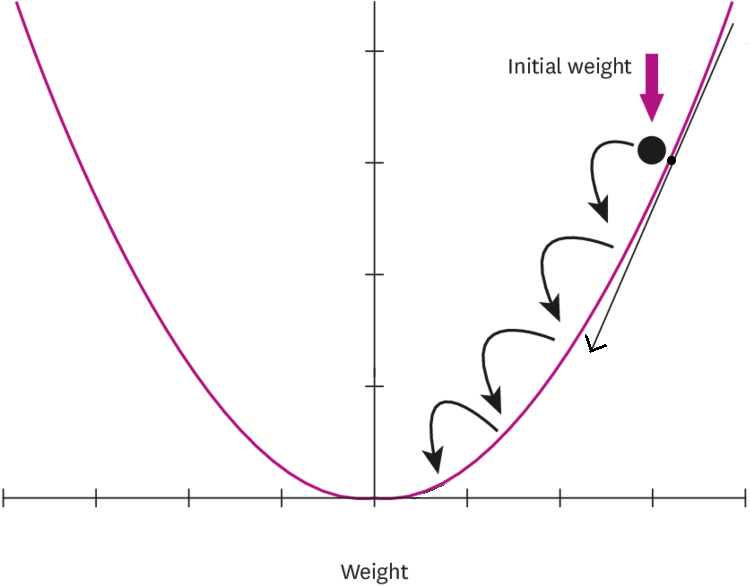
\includegraphics[scale=0.4]{MSE}
    \caption{The MSE of a perceptron with one input node}
\end{figure}

\vskip 0.2cm

\noindent
As Figure 15 shows the local minimum of the MSE and finding a weight $w$ such that the loss function is at the local minimum is equivalent to minimizing the error, which is desired as described in section 4.4.1. One way of finding that local minimum is to descend the loss function by using its slope at the current weight, also known as the derivative at that point. Note that we assume that the loss function is defined and differentiable around that point. Since the slope describes the 'steepness' of the loss function in the current point, following the direction of that slope will either lead you to a local maximum or minimum. It could be thought of as walking up or down a hill as illustrated by Figure 15 above. The slope of the MSE changes as one walks down the slope, assuring that the movement is towards the minimum. This type of descent will be described more rigorously in the following sections.

\newpage

\subsubsection{Gradient}

\vskip 0.2cm

In order to rigorously generalize the descent algorithm described in section 4.4.2 a new mathematical tool needs to be introduced. Namely the \emph{gradient} of a function. The example used in section 4.4.2 was a perceptron with a single output node and a single input node. Having a multilayer neural network with several weight connections instead leads to the loss function being dependant on several variables, namely the weights $w_{1}, w_{2}, ..., w_{n}$. To find the slope of a function $f(w_{1}, w_{2}, ..., w_{n})$ in a point we employ a mathematical technique called \emph{partial derivatives}. Let us use a small example. Take the following simple case of $f$: 

\vskip 0.5cm

\centerline{$f(w_{1}, w_{2}) = (w_{1} - w_{2})^2 = w_{1}^2 - 2w_{1}w_{2} + w_{2}^2$}

\vskip 0.5cm

\noindent
In order to use any kind of derivate we need to focus on one variable at a time, treating the others as unknown constants. Taking the partial derivative of $f$ with respect to $w_{1}$ looks as follows:

\vskip 0.3cm

\centerline{$f'(w_{1}) = D_{w_{1}}(w_{1}^2 - 2w_{1}w_{2} + w_{2}^2) = D_{w_{1}}(w_{1}^2) - D_{w_{1}}(2w_{1}w_{2}) + D_{w_{1}}(w_{2}^2) =$}

\vskip 0.3cm

\centerline{$2w_{1} - 2w_{2} + 0 = 2(w_{1} - w_{2})$}

\vskip 0.3cm

\noindent
The partial derivative $f'(w_{1})$ we calculated is correctly denoted as $\frac{\delta f(w_{1}, w_{2})}{\delta w_{1}} = 2(w_{1} - w_{2})$. Furthermore, just as $f(w_{1}, w_{2})$ has a partial derivative with respect to $w_{1}$ it also has a partial derivative with respect to $w_{2}$: $\frac{\delta f(w_{1}, w_{2})}{\delta w_{2}} = 2(w_{2} - w_{1})$. So if we now return to our original loss function $f(w_{1}, w_{2}, ..., w_{n})$ it would have $n$ partial derivatives $\frac{\delta f(w_{1}, ..., w_{n})}{\delta w_{1}}, \frac{\delta f(w_{1}, ..., w_{n})}{\delta w_{2}}, ..., \frac{\delta f(w_{1}, ..., w_{n})}{\delta w_{n}}$. If we now store those partial derivatives in an $n$-dimensional vector we get the following:

\vskip 0.5cm 

\centerline{\scalebox{1.4}{$[\frac{\delta f(\mathbf{w})}{\delta w_{1}}, \frac{\delta f(\mathbf{w})}{\delta w_{2}}, ..., \frac{\delta f(\mathbf{w})}{\delta w_{n}}]$}}

\vskip 0.5cm

\noindent
This structure is called the \emph{gradient} of the function $f(\mathbf{w})$ and is written as $\triangledown f(\mathbf{w})$, where $\mathbf{w}$ denotes the vector of arguments $[w_{1}, w_{2}, ..., w_{n}]$ taken in by the function $f$. A function, such as $f$, that takes $n$ arguments lives in an $(n+1)$-dimensional space and the gradient then simply becomes a list of derivates or slopes in each of the directions. Since each component of the gradient tells how fast the function $f$ is changing relative to the standard basis, it is natural to wonder, how fast the function $f$ might be changing relative to an arbitrary direction. Letting $\vv{v}$ denote a unit vector, we can project the gradient along this direction via the dot product as follows:

\vskip 0.5cm

\centerline{$\triangledown f(\mathbf{w}) \cdot \vv{v} = |\triangledown f(\mathbf{w})||\vv{v}|\cos(\theta) = |\triangledown f(\mathbf{w})|\cos(\theta)$}

\vskip 0.5cm

\noindent
Since the dot product is maximum when $\cos(\theta) = 1$, it is in particular maximum when $\vv{v}$ points in the same direction as the gradient of $f$, $\triangledown f(\mathbf{w})$. Furthermore, since the dot product is a projection of the gradient along the direction of $\vv{v}$ it implies that the rate of change of $f$ is maximal in the direction of the gradient, which conversely implies that $\triangledown f(\mathbf{w})$ points in the direction of the steepest ascent. The steeped descent of $f$ at $\mathbf{w}$ is then $-\triangledown f(\mathbf{w})$.

\newpage

\subsubsection{Gradient Descent}

\vskip 0.2cm

\noindent
Just as the derivative was used in a previous section $(4.4.2)$ to descend the MSE in the 2-dimensional space, the gradient described in the preceding section is used to descend a multi-variable loss function $f(\mathbf{x})$ to find a local minimum. The algorithm is called \emph{Gradient Descent} \cite{skansi} and is based on the fact, described in section 4.4.3, that if the multi-variable function $f(\mathbf{x})$ is defined and differentiable around a point $\mathbf{w}$, then $f(\mathbf{x})$ decreases quickest if one moves from $\mathbf{w}$ in the direction of the negative gradient of $f$ at $\mathbf{w}$, $-\triangledown f(\mathbf{w})$. The algorithm is formally defined as follows:

\vskip 0.3cm

\begin{figure}[h]
    \centerline{\scalebox{1.3}{$\mathbf{w}_{n+1} = \mathbf{w}_{n} - \gamma\triangledown f(\mathbf{w}_{n})$}}
    \vskip 0.2cm
    \caption{The Gradient Descent algorithm}
\end{figure}

\vskip 0.3cm

\noindent
For a small enough learning rate $\gamma \in \mathbb{R}_{+}$, then  $f(\mathbf{w}_{n+1}) \leq f(\mathbf{w}_{n})$. If one, with this observation in mind, starts at a point $\mathbf{w}_{0}$ and considers the sequence $\mathbf{w}_{0}, \mathbf{w}_{1}, \mathbf{w}_{2}, ...$ such that the recursive algorithm in Figure 16 holds, then we get the following monotonic sequence:

\vskip 0.5cm

\centerline{$f(\mathbf{w}_{0}) \geq f(\mathbf{w}_{1}) \geq f(\mathbf{w}_{2}) \geq f(\mathbf{w}_{3}), ...$}

\vskip 0.5cm

\noindent
The idea is then that the sequence will converge \cite{skansi} to a local minimum, which is what we are trying to find on the loss function as described in section 4.4.1. To grasp the intuition behind gradient descent, let us imagine a hypothetical scenario. A person is somewhere in the mountains and is trying to reach the bottom (i.e., trying to reach the global minimum). Due to heavy fog, the path down the mountain is not visible to the person and they must instead use local information to find the minimum. They can use the gradient descent algorithm by looking at the steepness of the hill at their current location and choosing the direction with the steepest descent. Eventually, the person would move, converge, to the bottom of the mountain, the global minimum, or possibly get stuck in a hole or a cave, the local minimum.

\begin{figure}[h]
    \center
    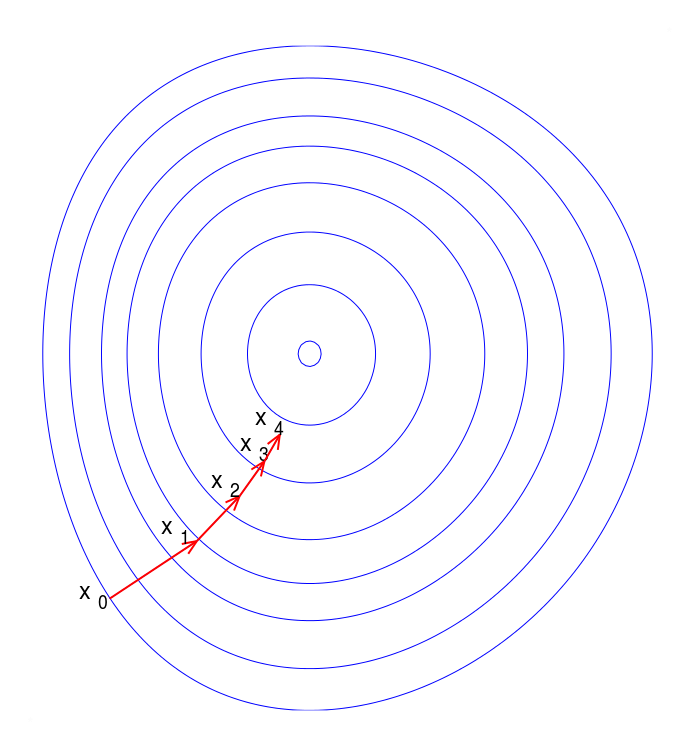
\includegraphics[scale=0.191]{gradientdescent}
    \caption{\scriptsize Illustration of the gradient descent algorithm}
\end{figure}

\newpage

\subsubsection{Backpropogation}

\vskip 0.2cm

We now have the necessary tools in order to train a neural network. As mentioned in section 4.3 we seek to adjust the weight connections of the network in order to make it the statistical model we seek. Sections 4.4.2 to 4.4.4 further explain that we train the neural network by finding the minima of a loss function, which we in turn do by adjusting the weight connections with an algorithm called gradient descent (4.4.4). In the single-layer perceptron, the loss function can be computed as a direct function of the weights, which allows easy gradient computation. In the case of multi-layer neural networks, it becomes a lot harder since the loss function is a complicated composition function of the weights throughout the hidden layers and several non-linear activation functions. The gradient of a composition function leverages the chain rule of differential calculus since the gradient simply is a vector of partial derivatives. Using the chain rule throughout all paths from the output to the input to get the partial derivatives relative to each weight connection takes an exponential amount of computations due to the exponential amount of paths. This is on the other hand possible to avoid using \emph{dynamic programming} \cite{charu}. The \emph{backpropagation} algorithm \cite{charu} described in this section is a direct application of dynamic programming. It consists of two phases, the \emph{forward pass} and the \emph{backward pass}:

\begin{outline}
    \1 \emph{Forward pass:} The input values for a training instance are fed into the neural network which leads to multiple forward computations across the layers using the current weight connections of the network. The final output of the neural network is then compared to the output target of the training instance with a chosen loss function. The partial derivatives of the loss function now need to be computed with respect to each weight connection in the network in the backward pass. This pass also stores specific information which will be used in the backward pass.
    \1 \emph{Backward pass:} In this pass, the gradient of the loss function is calculated with respect to the different weights in the neural network by using the chain rule of differential calculus. The partial derivatives in the gradient are then used to adjust or update the weights as described in section 4.4.4. Since dynamic programming is used to find the partial derivatives efficiently, the backward pass needs to start from the output layer and move in the backward direction, hence the name of the pass.
\end{outline}

\noindent
Consider a path of nodes where $v_{1}, v_{2}, ..., v_{k}$ both denote the nodes and the values sent forward by them to produce the network output $o$. Furthermore, let the weight connection between nodes $i$ and $i+1$ be denoted as $w_{(i, i+1)}$. Then, by using the chain rule follows \cite{charu} one can derive the gradient of the loss function, $L$, with respect to any of the edges, $w_{(i, j)}$, in the path as follows:

\vskip 0.3cm

\begin{figure}[h]
    \centerline{\scalebox{1.6}{$\frac{\delta L}{\delta w_{(i-1, i)}} = \frac{\delta L}{\delta o} [\frac{\delta o}{\delta v_{k}} \prod_{j=i}^{k-1} \frac{\delta v_{j+1}}{\delta v_{j}}] \frac{\delta v_{i}}{\delta w_{(i-1, i)}}$}, $\forall i \in 1 ... k$}
    \vskip 0.3cm
    \caption{Computing the gradient of the loss function with respect to a weight connection which only has a single path to the output $o$ in the neural network}
\end{figure}

\newpage

\noindent
The above expression assumes that there only exists a single path from the node $v_{1}$ to $o$ in the neural network, even though an exponential number of such paths might exist. A generalization of the chain rule used above in Figure 18, referred to as the \emph{multivariable chain rule}, can compute the gradient of the loss function with respect to a weight connection that has more than one path to $o$. It is done by adding the compositions along the paths from the node $v_{1}$ to $o$ \cite{charu}. Let $P$ be the set of paths from the node $v_{1}$ to $o$. The generalization of the expression in Figure 18 becomes as follows \cite{charu}:

\vskip 0.3cm

\begin{figure}[h]
    \centerline{\scalebox{1.6}{$\frac{\delta L}{\delta w_{(i-1, i)}} = \underbrace{\frac{\delta L}{\delta o} [\sum_{[v_{i}, v_{i+1}, ..., v_{k}, o] \in P}\frac{\delta o}{\delta v_{k}} \prod_{j=i}^{k-1} \frac{\delta v_{j+1}}{\delta v_{j}}]}_\text{$\triangle (v_{i}, o) = \frac{\delta L}{\delta v_{i}}$}\frac{\delta v_{i}}{\delta w_{(i-1, i)}}$}}
    \vskip 0.3cm
    \caption{Computing the gradient of the loss function with respect to a weight connection which has a set of paths, $P$, to the output $o$}
\end{figure}

\vskip 0.3cm

\noindent
The computation of the term $\frac{\delta v_{i}}{\delta w_{(i-1, i)}}$ on the right-hand side of the equation in Figure 19 is quite simple and is discussed below. The term $\triangle (v_{i}, o)$ is however computed over an exponentially increasing number of paths which at first sight seems quite troublesome. This is where dynamic programming is used and it is based on the insight that the graph of a neural network does not have any cycles, it is acyclic. Dynamic programming, simply put, employs a certain order of computing in order to reduce the number of computations necessary. By first computing $\triangle (v_{i}, o)$ for nodes $v_{i}$ with direct connections to the output $o$ and then recursively computing these values for nodes in earlier layers in terms of values in later layers we reduce the number of computations. Since we this way never recompute the gradient for a node or a connection, the number of computations becomes the number of nodes plus the number of connections in the network. The time complexity is in other words $O(E + V)$, where $E$ and $V$ are the numbers of edges and nodes in the graph representation of the network, respectively. In summary, the dynamic programming technique allowed us to reduce the number of computations from an exponential to a linear amount thanks to the acyclic property of the neural network. The recursion for $\triangle (v_{i}, o)$ using dynamic programming can be defined using the multivariate chain rule as follows:

\vskip 0.3cm

\begin{figure}[h]
    \centerline{
        \scalebox{1.2}{
            $
            \begin{cases} 
                \triangle (o, o) = \frac{\delta L}{\delta o} \\
                \triangle (v_{i}, o) = \frac{\delta L}{\delta v_{i}} = \sum_{v: v_{i} \Rightarrow v} \frac{\delta L}{\delta v} \frac{\delta v}{\delta v_{i}} = \sum_{v: v_{i} \Rightarrow v} \frac{\delta v}{\delta v_{i}} \triangle (v, o)
            \end{cases}
            $
        }
    }
    \vskip 0.3cm
    \caption{Computing $\triangle (v_{i}, o)$ recursively using dynamic programming}
\end{figure}

\vskip 0.2cm

\noindent
Since each $v$ is in a later layer than $v_{i}$, the term $\triangle (v, o)$ on the right-hand side has already been computed. The only thing left to evaluate for the computation is the term $\frac{\delta v}{\delta v_{i}}$. Let the weight connection between $v$ and $v_{i}$ be denoted as $w_{(v_{i}, v)}$ and let $v'$ be the value in node $v$ just before its activation function, $\Phi(\cdot)$, has been applied. By using earlier definitions in this section, we have that $v = \Phi(v')$ and by the chain rule \cite{charu}, the following expression for $\frac{\delta v}{\delta v_{i}}$ can be derived:

\vskip 0.2cm

\begin{figure}[h]
    \centerline{\scalebox{1.4}{$\frac{\delta v}{\delta v_{i}} = \frac{\delta v}{\delta v'} \frac{\delta v'}{\delta v_{i}} = \frac{\delta \Phi(v')}{\delta v'} w_{(v_{i}, v)} = \Phi'(v') w_{(v_{i}, v)}$}}
    \vskip 0.2cm
    \caption{Computing $\frac{\delta v}{\delta v_{i}}$}
\end{figure}

\vskip 0.3cm

\noindent
Using the expression in Figure 21 in combination with the expression in Figure 20 the following recursion is attained:

\vskip 0.3cm

\begin{figure}[h]
    \centerline{
        \scalebox{1.2}{
            $
            \begin{cases} 
                \triangle (o, o) = \frac{\delta L}{\delta o} \\
                \triangle (v_{i}, o) = \sum_{v: v_{i} \Rightarrow v} \Phi'(v') w_{(v_{i}, v)} \triangle(h, o)
            \end{cases}
            $
        }
    }
    \vskip 0.3cm
    \caption{Computing $\triangle (v_{i}, o)$ recursively using dynamic programming}
\end{figure}

\vskip 0.2cm

\noindent
Using the recursive formula in Figure 22, gradients are successively calculated in the backwards direction, and each node and edge in the neural network is processed exactly once in the backwards pass. Finally, the computation of the term $\frac{\delta v_{i}}{\delta w_{(i-1, i)}}$ is necessary for the expression in Figure 19. The computation can be done as follows:

\vskip 0.3cm

\begin{figure}[h]
    \centerline{\scalebox{1.4}{$\frac{\delta v_{i}}{\delta w_{(i-1, i)}} = v_{i-1} \Phi'(v_{i}')$}}
    \vskip 0.3cm
    \caption{Computing $\frac{\delta v_{i}}{\delta w_{(i-1, i)}}$}
\end{figure}

\vskip 0.2cm

\noindent
Every term in the expression in Figure 19 is now computable with the expressions in Figures 22 and 23, which themselves are computable with values that are gathered and saved during the forward pass. We can now efficiently calculate the gradient of the loss function with respect to every weight connection, which then can be adjusted by the gradient descent algorithm, described in section 4.4.4, for each available training instance (each training instance being some input values and their corresponding output targets).

\newpage

\subsection{Convolutional Neural Network}

\epigraph{
\vskip 0.5cm
\hspace{1.4cm} In order to carry a positive action we must develop here a positive vision.
}
\vskip -0.2cm
\centerline{\scriptsize --Dalai Lama}

\subsubsection{Historical Background}

\vskip 0.2cm

In this section, we introduce the convolutional neural network, which was invented by Yann LeCun and others in 1988 \cite{lecun}. Lecun and his team implemented ideas of David H. Hubel and Torsten Weisel present in their 1968 seminal paper \cite{skansi} which won them the 1981 Nobel Prize in Physiology and Medicine. They discovered the \emph{receptive field}, which describes the link between parts of the visual fields and individual neurons in the brain that process the information. 

\subsubsection{Architecture of a Convolutional Network}

\vskip 0.2cm

A convolutional neural network \cite{skansi} is a neural network that consists of one or more convolutional layers. A convolutional layer \cite{skansi} takes an image, a 2-dimensional grid with values, as input and passes a local receptive field, also known as \emph{kernel}, over the whole image. The kernel is a square grid with weights in each cell and starts in the top left corner of the input image and proceeds to move stepwise from left to right, row by row. At each place the kernel visits, it computes a value for the output image by adding all of the weights multiplied by their corresponding value in the input image, a weighted sum. One thing to notice is that the output image will be smaller than the input image. If we use a 3 by 3 local receptive field to scan a 17 by 8 image, we will get a 15 by 6 output image. Getting the image smaller means packing the information in a more compact and deeper representation, which is computationally beneficial. This whole process is illustrated in Figure 24 \cite{skansi} below. 

\vskip 0.3cm

\begin{figure}[h]
    \center
    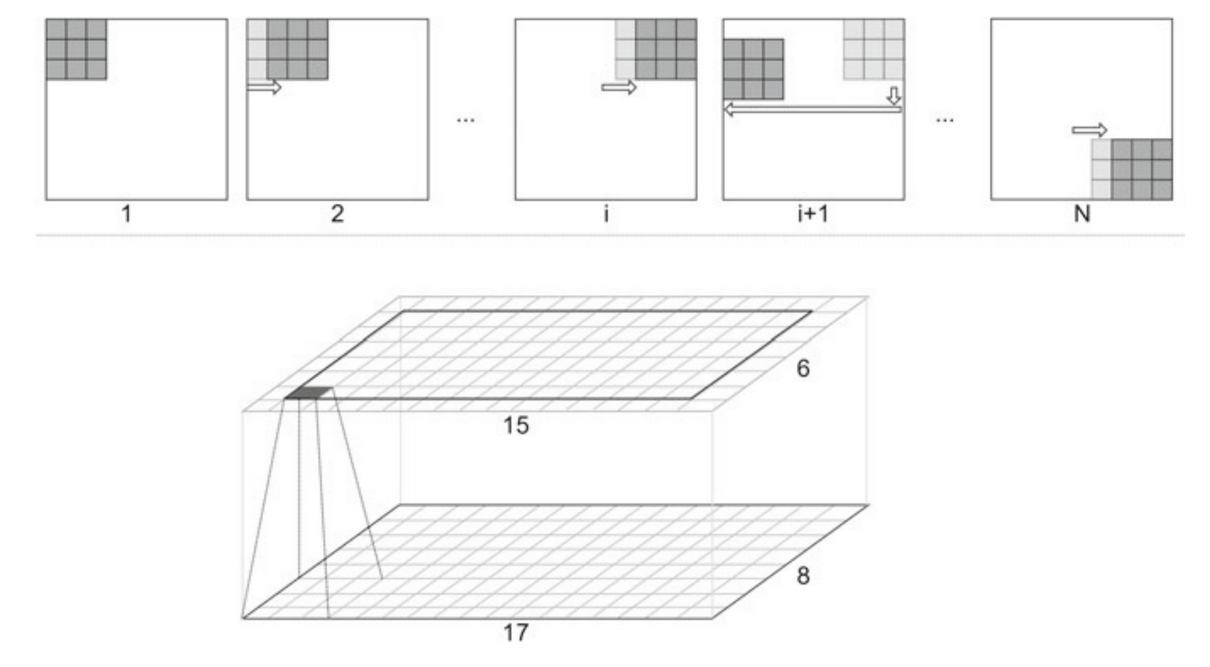
\includegraphics[scale=0.3]{kernel}
    \vskip 0.2cm
    \caption{A convolutional layer performing a scan of a 17 by 8 input image with a 3 by 3 local receptive field, creating a 15 by 6 output image}
\end{figure}

\newpage

\subsubsection{Intuition}

\vskip 0.2cm

One might wonder why the local receptive field of a convolutional layer is useful and the intuition behind it is quite simple. In a standard multilayer neural network, each input value is fed into the network independently and undergoes a handful of different computations. This assumes that there are no important correlations between the input value since they are fed into the network separately. That is however in reality often not the case. Our board game Connect Four (section 2) is an example of this phenomenon. A simple multilayer neural network would simply read each cell in the Connect Four grid individually and would lose important correlations such as 3 tokes of the same color being in a line. A 4 by 4 local receptive field of a convolutional layer on the other hand would create a weighted sum for each 4 by 4 square on the Connect Four grid. Each of those weighted sums could then give information about, for example, whether there are 3 tokens of the same color in a line anywhere or not. One could say that the local receptive field notices "the larger picture". 

\vskip 0.2cm

\noindent
The idea of collecting information about various correlations in an input image by using a local receptive field can be further improved. Instead of using a single local receptive field in a convolutional layer, one can use several, each of the same size but initialized with varying weights. We pass each local receptive field independently over the input image and create as many output images as there are receptive fields. Feeding a 10 by 10 image into a convolutional layer with 3 4 by 4 kernels would create 3 7 by 7 output images. We say that the output image has 3 \emph{channels}. The intuition behind having several kernels is that we increase the probability that one of the kernels "sees" an important correlation, which in turn increases the overall performance of the network. Figure 25 below illustrates this concept of channels.

\vskip 0.4cm

\begin{figure}[h]
    \center
    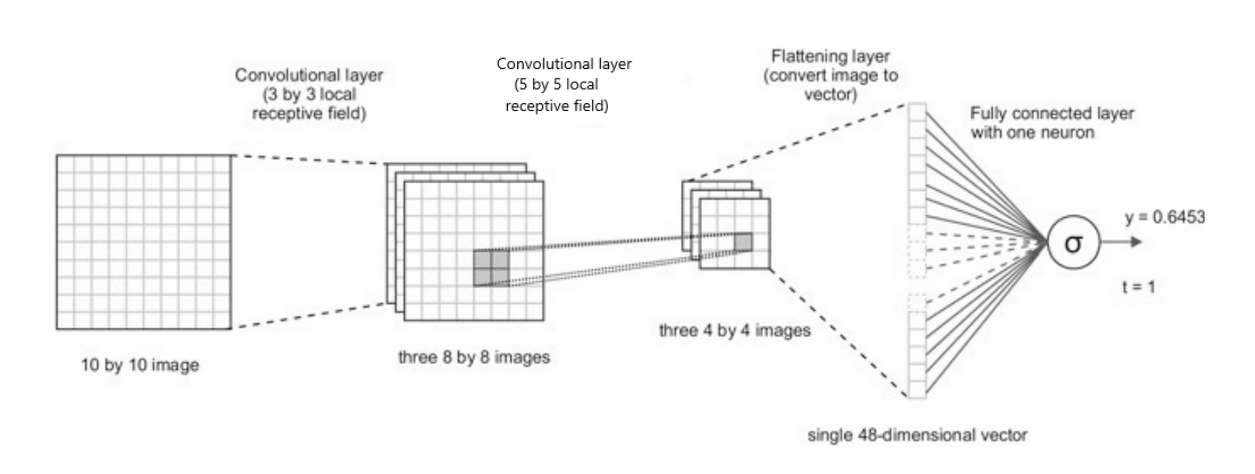
\includegraphics[scale=0.36]{cnet}
    \vskip 0.4cm
    \caption{A convolutional neural network with 2 convolutional layers followd by a fully connected layer}
\end{figure}

\vskip 0.2cm

\noindent
As shown in Figure 25, a convolutional neural network ends with fully connected layers, where the first one takes the output image of the preceding convolutional layer converted into a 1-dimensional vector as input. The same backpropagation algorithm, section 4.4.5, is then used to train the network, as for a standard multilayer neural network.

\newpage

\section{Heuristic Algorithms}

\vskip 0.3cm

The word \emph{heuristic} comes from Greek and means "To discover". It is in computer science a technique designed for solving a problem more quickly when the usual methods are too slow for finding an approximate solution or fail to find any exact one. It is achieved by trading optimality, completeness, accuracy, or precision for speed and could be considered a "shortcut". The following section describes the heuristic algorithm Monte Carlo Tree Search, which was used to test the performance of our neural networks. We will only describe the algorithm briefly and it is not necessary to fully understand it.

\subsection{Monte Carlo Tree Search}

\vskip 0.2cm

Let us consider the search tree of Connect Four. The root of the tree is the current board state the player is in. For each state reachable from the root by making a single move we create a child node to the root. We then recursively expand from each of those child nodes and get what we call a search tree. Since this tree expands exponentially, exploring every path from the root to a leaf node, where the game terminates, would take too much time. This is where the \emph{Monte Carlo Tree Search}, MCTS, excels since it heuristically chooses the paths of what it deems the most promising moves, effectively reducing the search space. The MCTS is based on many roll-outs, in which each is a game played out to the end by heuristically choosing moves. The outcome of each game is then used to weight the nodes in the search tree in order to favor better moves in the future. The way we used the MCTS was to let it use a certain amount of roll-outs for each board state and then choose the move which led to the most wins in the roll-outs. The following describes a roll-out of the Monte Carlo Tree Search \cite{mcts}:

\begin{outline}
    \1 \emph{Selection:} Start from root $R$, the current game state, and heuristically select child nodes until a leaf node $L$ is reached. A leaf might either be a terminated game state or a state that has not been further explored by the MCTS. 
    \1 \emph{Expansion:} Unless $L$ is the end of the game, create all possible child nodes from $L$ and choose node $C$ from one of them.
    \1 \emph{Simulation:} Complete one random game from node $C$.
    \1 \emph{Backpropagation:} Use the result of the game from node $C$ in order to update the information in the nodes on the path from $C$ to $R$.
\end{outline}

\vskip 0.2cm

\noindent
The selection of child nodes during the selection phase is in our MCTS done using an expression called \emph{Upper Confidence Bound} \cite{ucb}, which will not be described in this paper. Note that we will refer to Monte Carlo Tree Search with $n$ roll-outs per move as MCTS-$n$.

\newpage

\section{Method}

\vskip 0.3cm

\epigraph{
\hspace{3.07cm} A goal is only a mean to start a process.
}
\vskip -0.2cm
\centerline{\scriptsize --Adam Amanbaev}

\subsection{Implementation}

\vskip 0.2cm

Everything used in this project, except tools for plotting data, was implemented using the programming language C++. We implemented several neural networks that each trained to play the board game Connect Four, described in section 2. By then comparing the game performance of the various networks, we could analyze the impact their varying parameters have, as described in section 1.2. The game performance was measured by the percentage of wins, \emph{winrate}, in Connect Four.

\vskip 0.2cm

\noindent
Our convolutional neural networks take the Connect Four board as a 6 by 7 input image where each cell contains a value of $-1, 0, $ or $1$ if there is a black token, white token or no token there, respectively. The network's output layer consists of 7 output nodes. One for every column a token can be dropped in the Connect Four board. Each of the output nodes is a value function that evaluate the corresponding move. Greater values signify better moves and lower values signify worse moves.

\vskip 0.2cm

\noindent
Each convolutional neural network we trained in this project had a set of parameters that were the same across all of them. Each network began with a convolutional layer consisting of 256 kernels. In other words, a convolutional layer that outputs an image with 256 channels. The convolutional layer is afterwards, in each network, followed by 3 fully connected layers containing 64, 64 and 7 nodes each.

\subsection{Training}

\vskip 0.2cm

The training of our neural networks was done by \emph{self-play}. Each neural network played several games, each called an epoch, against itself where each move it made was recorded. The networks were then after each game trained using backpropagation in order to approximate the Q-function in Q-learning or double Q-learning, described in sections 3.5 and 3.6. Each training instance consisted of the moves made by the neural network and whether they in the end led to a win or a loss. The moves that directly led to a loss or a win, got the reward $R = -1$ or $R = 1$ in the Q-learning algorithm, respectively. Each neural network was trained for several hours during the night.

\newpage

\subsection{Benchmarking}

\vskip 0.2cm

As mentioned in section 6.1, we compared the neural networks by their game performances, which we define as the percentage of wins, and win rate, over a fixed number of games. In order to measure the game performance of the neural networks, we let them play against the heuristic algorithm Monte Carlo Tree Search over a set of 100 games each, after every 100 self-play training games. For each of the games played by the neural networks against a heuristic player, the number of wins draws and losses were recorded as well as the epoch the games were played after.

\vskip 0.2cm

\noindent
In order to compare the benchmarking data and draw conclusions about certain parameters, described in section 1.2, we made sure to create a batch of copies of a network for each parameter. For each network in a batch, we then varied the corresponding parameter to be able to analyze the impact that specific parameter has. One could say that we isolated each studied parameter in order to more efficiently draw conclusions.

\vskip 2cm

\begin{figure}[h]
    \center
    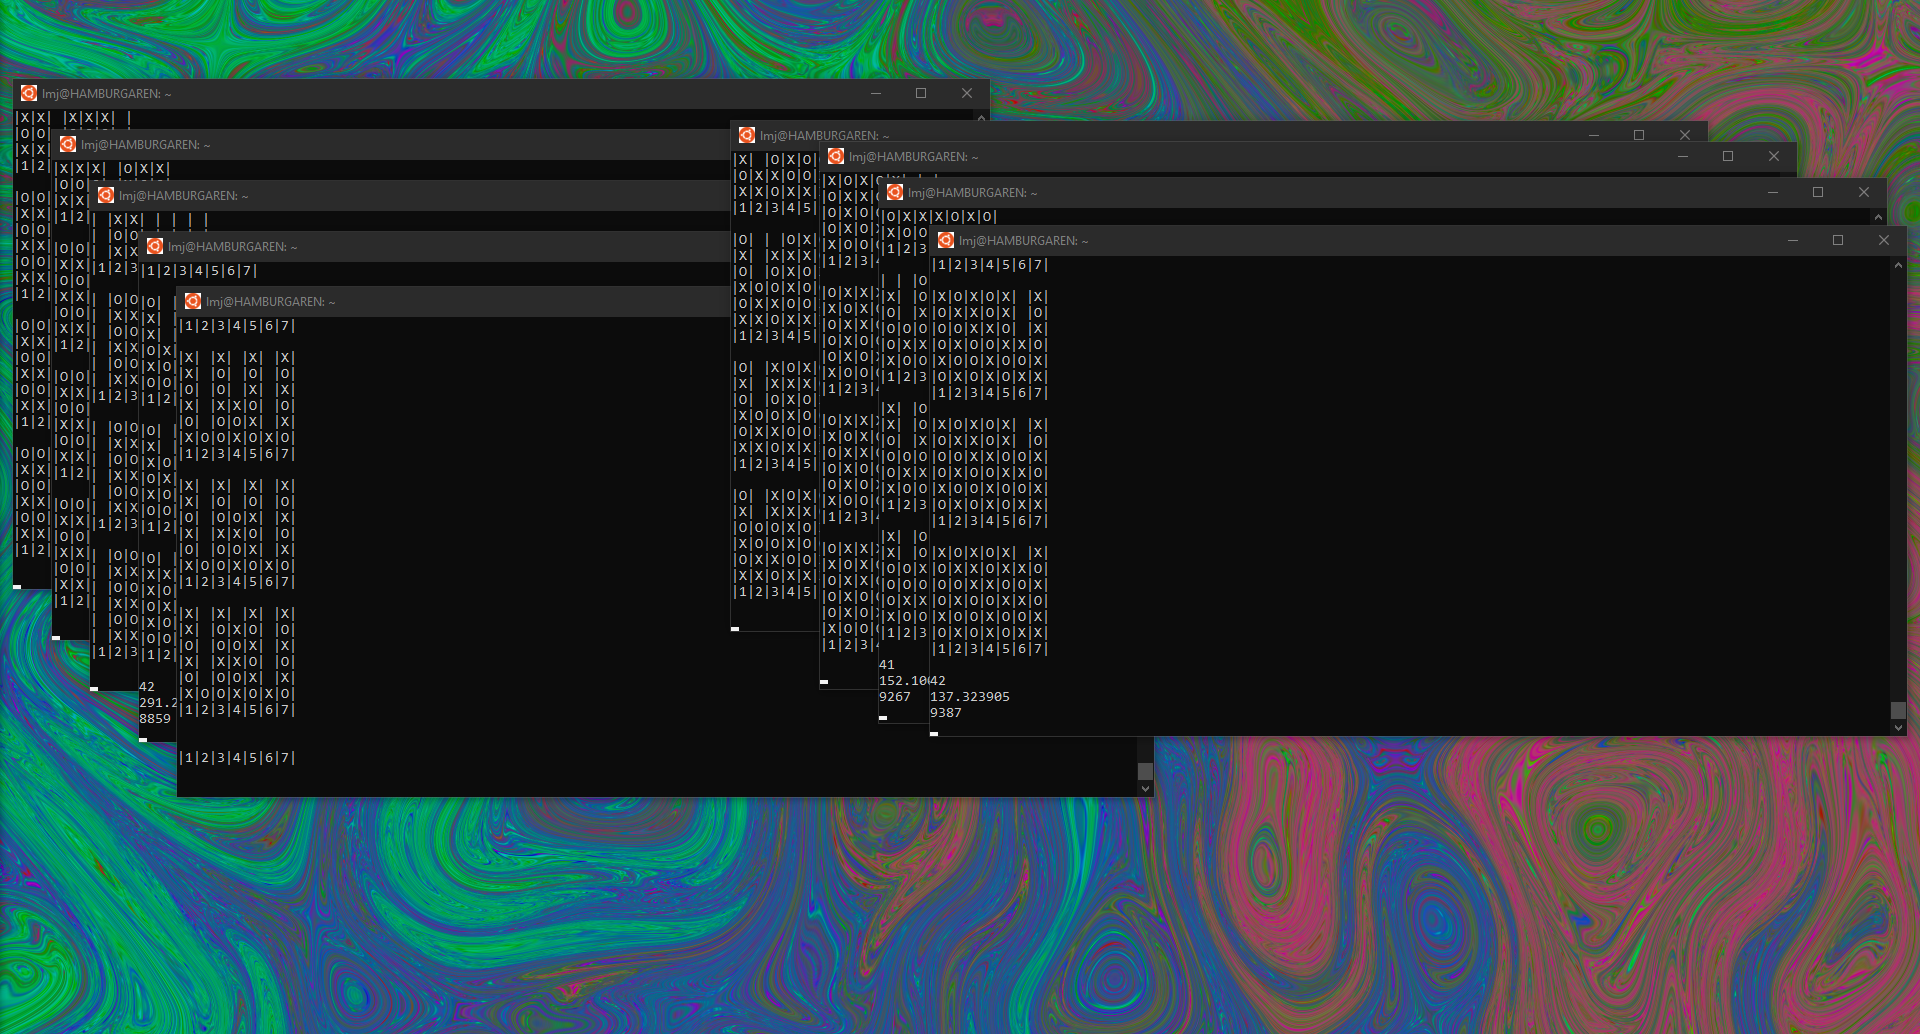
\includegraphics[scale=0.23]{nightrunning}
    \caption{Training and benchmarking several neural networks simultaneously during the night}
\end{figure}

\newpage

\section{Results and Analysis}

\subsection{Kernel Size}

\subsubsection{Results}

\vskip -0.7cm

\begin{figure}[h]
    \center
    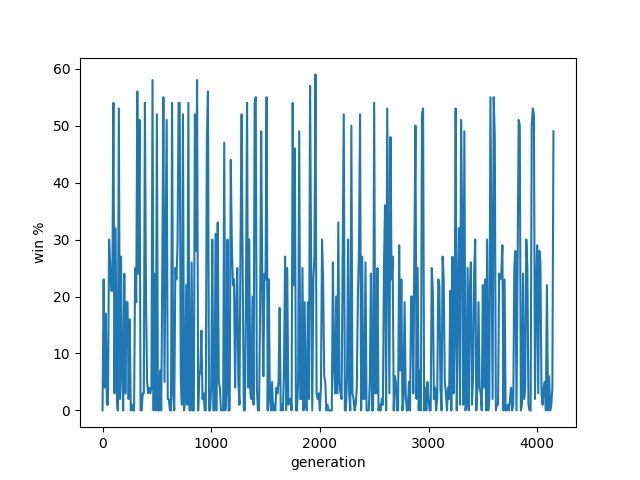
\includegraphics[scale=0.52]{Q-K5-L10-R5_vs_mcts2000}
    \caption{Convolutional neural network with kernel size 5 against MCTS-2000}
\end{figure}

\begin{figure}[h]
    \center
    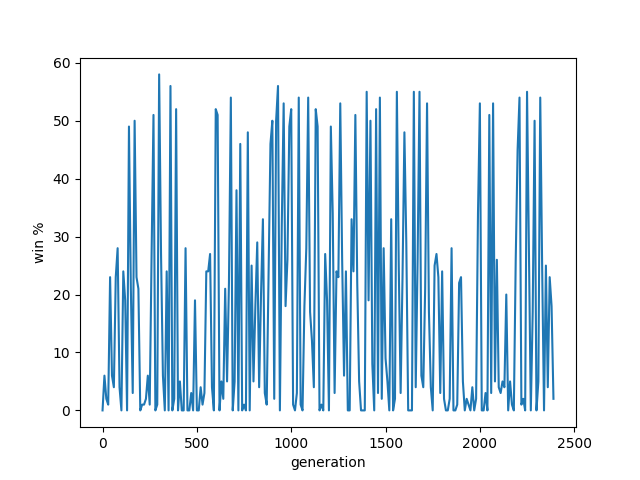
\includegraphics[scale=0.52]{DQ-K4-L10-R5_vs_mcts2000}
    \caption{Convolutional neural network with kernel size 4 against MCTS-2000}
\end{figure}

\newpage

\begin{figure}[h]
    \center
    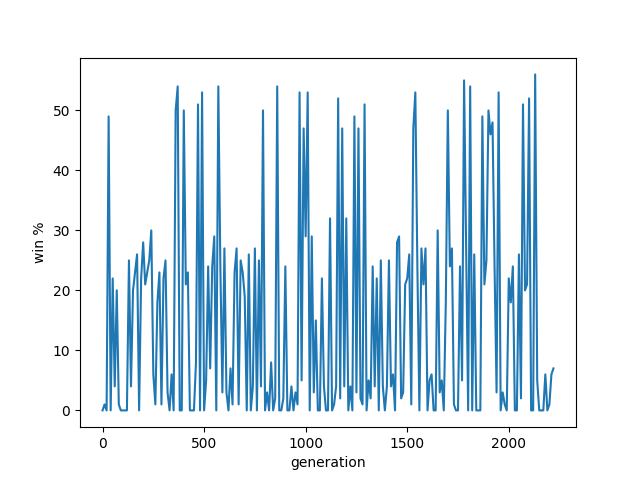
\includegraphics[scale=0.52]{Q-K2-L10-R5_vs_mcts2000}
    \caption{Convolutional neural network with kernel size 2 against MCTS-2000}
\end{figure}

\subsubsection{Analysis}

\vskip 0.5cm

Figures 27, 28 and 29 show graphs of the win percentage with respect to which generation of the neural network was playing. One generation is in this case equivalent to 100 epochs, with each epoch being a self-play training game. Each of the three neural networks was benchmarked against a Monte Carlo Tree Search player with a rollout limit set at 2000, where each data point is 100 games against it.

\vskip 0.2cm

\noindent
The first phenomenon noticeable in the data presented by the diagrams in Figures 27, 28 and 29, is \emph{catastrophic interference}, also referred to as \emph{catastrophic forgetting} \cite{catastrophic}. Notice the very sudden spikes in win rate for each of the neural networks followed by sudden drops in win rate. This pattern seems to repeat itself through the generations and it almost seems like the neural networks at some points learn how to win games but then suddenly forget what they have learnt. This is what we call catastrophic forgetting, which is defined as a tendency of a neural network to abruptly and drastically forget previously learnt information up learning new information \cite{catastrophic}. It is generally a challenge to create a neural network that is sensitive enough to detect small details, such as patterns in the Connect Four board, without being disrupted by new information \cite{catastrophic}. Catastrophic forgetting occurs when many of the weights that have been adjusted and learnt something, for example, the pattern of 3 tokens of the same color in a line, are changed by new data instances. It then becomes unlikely that the weights still "remember" what they had learnt previously since the latest information is being superimposed on top of the old information.

\vskip 0.2cm

\noindent
Furthermore, one can see that the neural networks with kernel sizes 4 and 5 in Figures 27 and 28 have win rates that more frequently reach a percentage of 50 and above in comparison with the convolutional network with kernel size 2. Figure 29 shows that the convolutional neural network with kernel size 2 generally spends a lot more time with a win rate of 30 percent and below when compared with the data in Figures 27 and 28. One could conclude that this is due to the 2 by 2 kernel, local receptive field, being a lot smaller than the 4 by 4 and 5 by 5 kernels. As described in section 4.5.2, the local receptive field is able to learn correlations in the input image. In our case, this enables the convolutional neural networks to learn and recognize patterns in the Connect Four board such as 3 tokes of the same color being in a line. That specific pattern is already quite important as it would be necessary to block such a line if it were of the opponent's color. Otherwise, the opponent could simply, if possible, complete that line and connect four of their tokens earning them a win. However, in order for a local receptive field to "spot" and recognize such a line of 3 tokens, it would need a size of at least 3. There is a possibility that the convolutional neural network with 2 by 2 local receptive fields simply could not learn such patterns and therefore performed worse than the networks with 4 by 4 and 5 by 5 receptive fields. Conversely, the convolutional networks with kernel sizes 4 and 5, respectively, were probably able to recognize such patterns a lot better and therefore also performed better against the opponent.

\subsection{Learning Rate}

\subsubsection{Results}

\begin{figure}[h]
    \center
    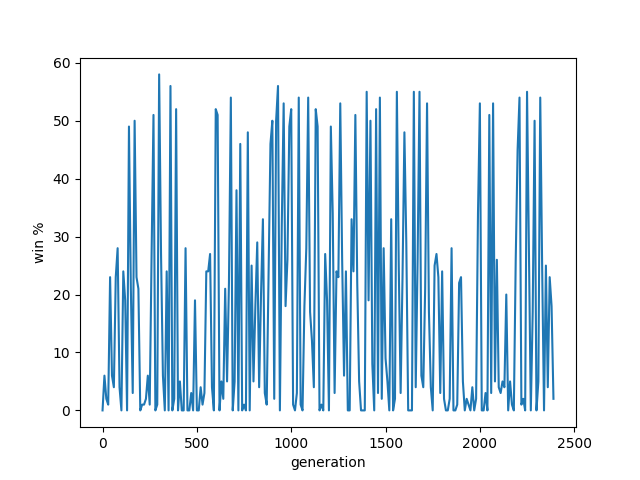
\includegraphics[scale=0.6]{DQ-K4-L10-R5_vc_mcts2000}
    \caption{Convolutional neural network trained using double Q-learning with learning rate 0.01 against MCTS-2000}
\end{figure}

\newpage

\begin{figure}[h]
    \center
    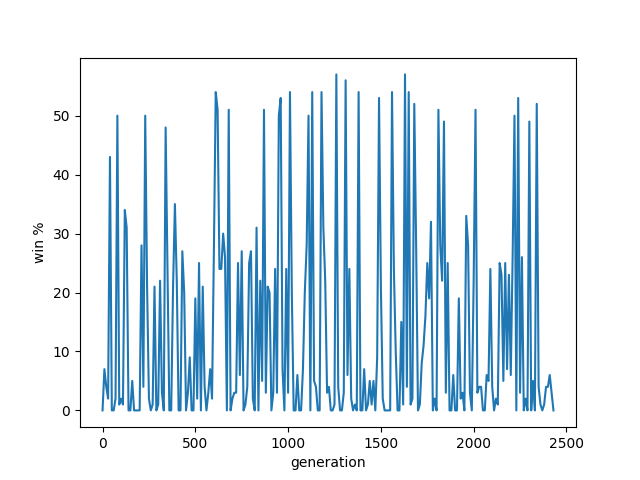
\includegraphics[scale=0.6]{DQ-K4-L200-R5_vc_mcts2000}
    \caption{Convolutional neural network trained using double Q-learning with learning rate 0.2 against MCTS-2000}
\end{figure}

\subsubsection{Analysis}

\vskip 0.2cm

Looking at the data presented in Figures 31 and 32, one can once again notice the phenomena called catastrophic forgetting, which is described above in section 7.1.2. However, there is interestingly a difference between the catastrophic forgetting in the neural network with a learning rate 0.01 in Figure 31 and in the network with learning 0.2 in Figure 32. As mentioned above, the forgetting is caused by the neural networks adjusting weights in order to learn new information when those weights had already been adjusted to learn previous information. Furthermore, as described in section 3.5, the learning rate is set to regulate the agent's, in this case, the neural network's, rate of learning in Q-learning or double Q-learning. The learning rate, in other words, regulates the rate of change in the weight connections in the neural network as it attempts to learn new information. This also implies that increasing the learning rate would encourage the neural network to change its weight connections in order to learn new information at hand which would in turn magnify the catastrophic forgetting. This can be seen when comparing the data in Figure 31 with the data in Figure 32. The win rate of the network with learning rate 0.2, shown in Figure 31, spends a lot more time around 30 percent and below while the win rate of the network with learning rate 0.01, shown in Figure 32, more frequently manages to increase beyond 30 percent to around 50 percent. A simple way to see this is by noticing that the graph in Figure 32 is densest in areas closer to 15 percent while the graph in Figure 31 is more dense in upper regions. Conversely, this also implies that decreasing the learning rate will reduce the amount of catastrophic forgetting since it discourages the network to readjust weight connections that possibly might already have "learnt" information.

\newpage

\subsection{Training Noise}

\subsubsection{Results}

\vskip -0.7cm

\begin{figure}[h]
    \center
    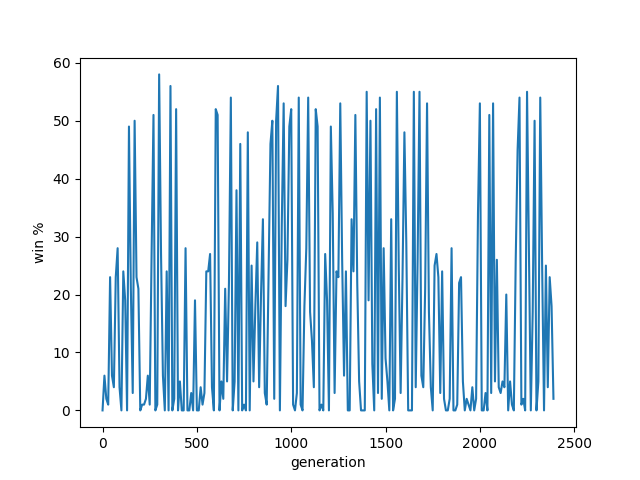
\includegraphics[scale=0.501]{DQ-K4-L10-R5_vs_mcts2000}
    \caption{\scriptsize Convlutional neural network trained using double Q-learning with training noise probability of 20 percent against MCTS-2000}
\end{figure}

\vskip 0.2cm

\begin{figure}[h]
    \center
    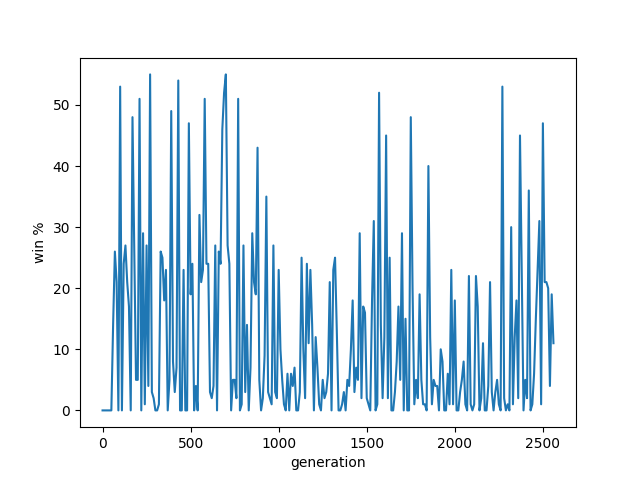
\includegraphics[scale=0.501]{DQ-K4-L10-R3_vs_mcts2000}
    \caption{\scriptsize Convlutional neural network trained using double Q-learning with training noise probability of \scalebox{0.7}{$(\approx)$} 33 percent against MCTS-2000}
\end{figure}

\newpage

\subsubsection{Analysis}

\vskip 0.2cm

\noindent
When training neural networks by self-play, meaning that the networks play against themselves, it is crucial to add what we would like to call \emph{training noise}. We define training noise as randomly forcing the networks to play random moves during their self-play training. The reason this is important is that we want the neural networks to reach new board states of Connect Four in order to learn new information about those states. Otherwise, the networks would simply repeat moves it had learnt at some point and never reach certain positions, which it later might lose due to lack of knowledge of it. However, forcing a network to play random moves during its training too often, might lead to the network exploring new board states too much instead of reinforcing good moves it had already learnt. It is therefore important to analyze how often training noise should be added and we thereby define the \emph{training noise probability} as the probability of a random move being forced upon a neural network during its self-play training. 

\vskip 0.2cm

\noindent
A higher training noise probability leads to the networks reaching new board states more frequently. In other words, it encourages the networks to explore and learn new information about the game, which in our case is Connect Four. Conversely, a lower training noise probability encourages the networks to repeat moves they have already learnt and thereby reinforce those moves if they are beneficial and often lead to wins. This kind of conflict between reaching new states in a Markov Decision Process (section 3.4) and reinforcing already learnt information, is often referred to as \emph{exploration} versus \emph{exploitation}.

\vskip 0.2cm

\noindent
However, since our neural networks are quite sensitive and prone to catastrophic forgetting, as mentioned previously, letting them explore and learn new information too much, would worsen their performance. This is noticeable in Figures 33 and 34 by looking at where each graph is densest, just as we did in section 7.7.2. The win rate of the graph in Figure 34 is densest closer to 10 percent which could imply that the network is frequently affected by catastrophic forgetting. This might be because it having a higher training noise probability which encourages the network to find and learn more new information, which in turn magnifies the catastrophic forgetting. The graph shown in Figure 33 is on the other hand denser in upper regions and reaches win-rates close to 55 percent a lot more frequently. This could imply that the network is not subjected to catastrophic forgetting as frequently as the network in Figure 34, which in turn could be due to the lower training noise probability of 20 percent. As mentioned above, a lower training noise probability will discourage the network from learning too much new information, which decreases catastrophic forgetting.

\newpage

\subsection{Possible Improvements of Method}

\vskip 0.2cm

One possible improvement of the method lies in the training of the neural networks. Since each network needs quite a lot of training hours in order to perform as well as possible, it would be beneficial to simply schedule more time for the training. Since each of us in the project needed to use our computers for school work, no neural network was able to train continuously for more than a night. One way to solve this problem could be by somehow getting access to another computer, perhaps from the school, which would be fully dedicated to training the neural networks. That way the networks could be trained for several days, which allows better data on the training progresses.

\subsection{Future Work}

\vskip 0.2cm

This paper studies the impact different parameters have on the learning of simple neural networks. In practice, most neural networks are significantly more complex and take a lot more time and better data to be trained well. It is then even more important to choose the parameters we present in this paper with care in order to improve the accuracy of the neural networks as well as minimise the amount of time spent training them. The results of this paper could therefore be used to train more sophisticated neural networks with more certainty and less time, which naturally aids the development and research of neural networks. A way to further develop this project, one could analyze how the parameters impact the performance of the neural networks when varied in combination with each other. A larger local receptive field of a convolutional neural network could for example benefit from a smaller learning rate in comparison to a smaller receptive field. Another way to continue this project would be by studying ways to prevent catastrophic interference, which our neural networks were subjected to quite often. 

\newpage

\bibliographystyle{unsrt}
\bibliography{refs}

\newpage

\appendix

\section{Appendix}
\subsection{Source Code}

\vskip 0.2cm

\centerline{The source code for this project can be found in the following github repository:}

\vskip 0.3cm

\centerline{\href{https://github.com/chopingu/hajar}{https://github.com/chopingu/hajar}}

\end{document}
